\section{Application}
\label{CH:Application}

The statistical characteristics of financial asset returns play a crucial role in today's economy. Risk assessment has become ever increasingly important given not only the recent history of financial markets\footnote{US-China trade war, corona virus outbreak, ...}. The financial crisis of 2007/2008, the burst of the 'dot com' bubble in the year 2000 and many other examples have shown that the financial market can cause major distress in banks, companies and for individual investors. The modeling of the first moment of the return distribution is important but for risk assessment, the most critical feature of the return distribution is its second moment, the variance, which has spurred a wide literature on forecasting and modeling of asset return characteristics. The following builds the foundation for the application of our model(s) to real world data.



\subsection{Mathematical Foundations}

The return process of a financial asset can be discribed by 
\begin{equation}
    r_{t+h} = P_{t+h} - P_t = \log{\tilde P_{t+h}} - \log{\tilde P_t}
\end{equation}
where $\tilde P_t$ is the price process of the asset. In the seminal work of \cite{Andersen2001DistributionofVola} and \cite{Andersen2003ModelForecastVola} they define the one-dimensional stochastic (Itô) process
\begin{equation}
    P_{t+h} - P_t = \int_{t}^{t+h} \mu_s \dd s + \int_{t}^{t+h} \sigma_s \dd B_s
\end{equation}

with a standard Brownian motion $B_t$, $\mu_s$ is a locally bounded and predictable dift process and $\sigma_s$ is the right-continuous and left-limit volatility. Given a sequence of partitions $\left(D_m\right)_{m\in\N}$ with $D_m = \left\{0 = t_1 < ... < t_m = T\right\}$ with $\sup_{1 \leq i \leq m} \abs{t_i - t_{i-1}} \to 0$ for $m \to \infty$, the quadratic variation $\langle P\rangle_t$ of $r_{t+h}$ is defined as
\begin{equation}
    \langle P\rangle_t = \lim_{m \to \infty} \sum_{\stackrel{t_i \in D_m}{t_i < t}} \left(P_{\text{min}\left(t_{i+1}, t\right)} - P_{t_i}\right)^2 \label{EQ:QuadraticVariation}
\end{equation}
which exists in probability. \cite{Billingsley2008} shows that
\begin{equation}
    \langle P\rangle_t = \int_{0}^{T} \sigma_s^2 \dd s \label{EQ:IntegratedVariance}
\end{equation}
which is known as integrated variance.

\subsection{Realized Volatility}
\label{CH:Application:RV}

\cite{NielsenShephard2004} were the first to introduce a consistent estimator for the integrated variance \refp{EQ:IntegratedVariance}\footnote{They even propose an estimator for integrated covariance.} under the assumption of no market microstructure noise\footnote{Market microstructure is concerned with the formation of the price and the 'noise' around it which arises from timing of transactions, flow and disclosure of information and the individual behaviour of market participants.}. Given the log-price process introduced earlier, they propose the Realized Volatility\footnote{The original papers were concerned with the Realized Variance but we will denote by $RV$ the Realized Volatility, so the square root of the Realized Variance.} $RV(0, t)$ as an estimator of the square root of the integrated variance by
\begin{equation}
    RV(0,t) = \sqrt{\sum_{j = 1}^{J} \left(P_{t_j} - P_{t_{j-1}}\right)^2} = \sqrt{\sum_{j = 1}^{J} r_{t_j}^2}
\end{equation}
given a partition $D_J = \left\{0 = t_0 < t_1 < ... < t_J = t\right\}$ for the period $\left[0, t\right]$. The defintion \refp{EQ:QuadraticVariation} implies the consistency of $RV(0,t)$, more precisely
\begin{equation}
    \text{p}\!\lim_{J \to \infty} RV(0,t)^2 = \int_{0}^{t} \sigma_s^2 \dd s
\end{equation}
The assumption of no market microstructure doesn't hold in reality due to multiple reasons. Firstly, the price of an asset is not continous but discrete with bounces between the bid-price and the ask-price. Secondly, the observation of prices is not continous but trades and as a consequence the new price happen irregularly. However, by design the estimator is positive and a compromise has to be found between market microstructure noise and consistency of the estimator.
\cite{Andersen2011MMN} give a detailed analysis of the effects of market microstructure noise on the estimation of realized volatility.

\subsection{Heterogeneous Autoregressive Model}

One of the most prominent models for the forecasting of realized volatility is the \textit{Heterogeneous Autoregressive model of Realized Volatility} (HAR) by \cite{Corsi2009}. He proposes an additive cascade model of volatility based on different time periods. It is a linear model and convices by its simplicity and its ability to reproducing the main empirical phenomena of financial returns (long memory, fat tails and self-similarity). It is often considered as a benchmark for the prediction of realized volatility and has proven itself to be hard to beat. \cite{Corsi2009} extends the daily realized volatility introduced in section \ref{CH:Application:RV} (now denoted by $\RVD_t$) to different time horizons longer than one day. By taking a simple average of the daily quantities he presents for example
\begin{equation}
    \RVW_t = \frac{1}{5}\left(\RVD_t + \RVD_{t-1} + \hdots + \RVD_{t-4}\right)
\end{equation}
to define a weekly realized volatility. Accordingly, he uses a average over the last $22$ days to define a monthly realized volatility $\RVM_t = \frac{1}{22}\sum_{i=0}^{21} \RVD_{t-i}$. The superscripts $(d)$, $(w)$ and $(m)$ refer to the time periods and subscript $t$ denotes the time. \cite{Corsi2009} mentions that the aggregate volatility over long time frames, as presented here, doesn't exactly represent the realized volatility over othe the specified time interval. The differences, he states, are immaterial and enable the interpretation of the model as a restricted AR(22) model of daily realized volatility. The specific choice of those time horizons can be motivated by dissimilarities in the approaches participants in financial markets. Endowments or pension funds - trading much less frequently - target a longer time horizon of their investments\footnote{Mostly even longer than one month.}, medium-term investors may rebalance their portfolios on a weekly basis, have different risk profiles and analyse markets on shorter timeframes, and day traders (as the name suggest), market makers or dealers look at daily timeframes. 
The overall emerging pattern is a volatility cascade from monthly (low) to daily (high) frequencies that builds the basis for a model with three heterogeneous volatility components.
Obviously, more components (quarterly or even yearly) could be added.
\cite{Corsi2009} defines the \textit{latent partial volatility} $\tilde \sigma_t^{(\cdot)}$ for three volatility components: one day $(d)$, one week $(w)$ and one month $(m)$. He argues that each component has an 'almost AR(1)' structure and that the shorter-term processes are influenced by the longer-term components to finally present:

\begin{eqnarray}
    \tilde \sigma_{t+1m}^{(m)} & = & c^{(m)} + \phi^{(m)}\RVM_t + \tilde \omega_{t+1m}^{(m)} \\
    \tilde \sigma_{t+1w}^{(w)} & = & c^{(w)} + \phi^{(w)}\RVW_t + \gamma^{(w)}\E{\tilde \sigma_{t+1m}^{(m)}} + \tilde \omega_{t+1w}^{(w)} \\
    \tilde \sigma_{t+1d}^{(d)} & = & c^{(d)} + \phi^{(d)}\RVD_t + \gamma^{(d)}\E{\tilde \sigma_{t+1w}^{(w)}} + \tilde \omega_{t+1d}^{(d)} \\
\end{eqnarray}

where $\RVM$, $\RVW$ and $\RVD$ are the (ex post) observed realized volatilities. The innovations $\tilde \omega_{t+1m}^{(m)}$, $\tilde \omega_{t+1w}^{(w)}$ and $\tilde \omega_{t+1d}^{(d)}$ are independent and appropriately left truncated error terms to ensure positiveness of the left-hand sides. Substitution of the partial processes of longer-term components into the daily component finally yields
\begin{equation}
    \RVD_{t+1d} = c + \beta^{(d)}\RVD_t + \beta^{(w)}\RVW_t + \beta^{(m)}\RVM_t + \omega_{t+1d} \label{EQ:HAR}
\end{equation}
A major drawback of \refp{EQ:HAR} is the fact, that the model doesn't guarantee positiveness of the $RV$ forecast. In order to remedy that, \cite{Corsi2009} suggests to work with the log-transformation of the realized volatility which practitioners almost always do.

\subsection{Methodology}
\label{CH:Application:Methodology}

The HAR model by \cite{Corsi2009} has the advantage that the model doesn't have any hyperparameters. One could use regularization techniques that have been presented in section \ref{CH:LinearRegression}, however due to the low dimensionality (in the general case, it only uses $3$ regressors and an intercept) the possibility of overfitting decreases as the amount of available data increases. With Echo State Networks that have multiple hyperparameters, the question arises on how to optimize those in order get decent predictive performance. There are many strategies and 

\subsubsection{Hyperparameter Optimization}
The choice of hyperparameters is a crucial step in the training of many machine learning models and has to be performed with due diligence.
In order to train our models and validate their hyperparameters, we are going to use k-fold cross-validation which has already been mentioned in section \ref{CH:LinearRegression}. Cross-validation describes the procedure of training a model on a subset of the available training data, which we will refer to as \textit{estimation set}, and validate its performance on another set of the data called \textit{validation set}, which hasn't been presented to the model in the estimation step. This simulates the situation when non-available data will be presented to the model in the future. Based on the error in the validation set, the hyperparameters of the model can be chosen in a reasonable way.
Many procedures have been presented that help to get a good representation of the performance of a model on unseen data, and we want to focus on two of those, namely a rolling window approach or an expanding window approach, which are presented in figure \refp{FIG:RollingExpanding}.
% Given a data set of size $T \in \N$, we will split the sample into a training set $S_{\text{train}} = \left\{0,...,t_{train}\right\}$ and a validation set $S_{\text{val}} = \left\{t_{train}+1,...,T\right\}$. To have a good representation of the performance on the validation set, one can choose two different approaches, namely a rolling window approach or an expanding window approach, which are presented in figure \refp{FIG:RollingExpanding}.
% Both approaches define a way of getting a estimate of the out-of-sample performance of a given set of hyperparameters. Instead of training just once on $S_{\text{train}}$ and validating on $S_{\text{val}}$, we estimate our model multiple times and average the out-of-sample performances. Define $\tau = \frac{T - \tau - 1}{k}$ which is assumed to be a natural number.
% For the moving window approach, define $S_{\text{train}}^k = \left\{k\tau,...,t_{train}+k\tau\right\}$ and a validation set $S_{\text{val}} = \left\{t_{train}+k\tau+1,...,t_{train}+(k+1)\tau\right\}$.



\begin{figure}
    \begin{center}
        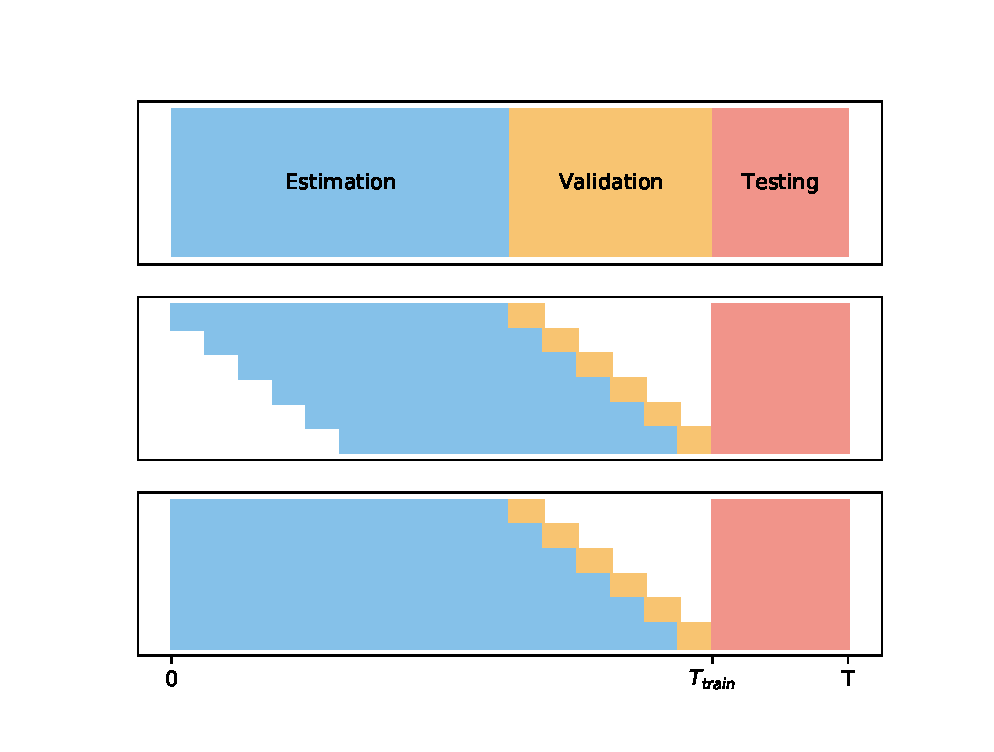
\includegraphics[width=\textwidth]{Plots/RollingExpandingWindow.eps}
    \end{center}
    \caption{The top panel describes the split of the avaliable data into an estimation and validation (which together is the training set) and a testing set, that is used to compare different models. The split was chosen $50\%$, $30\%$ and $20\%$, respectively. The center panel presents the rolling window approach and the expanding window approach is in the lower panel, both for a $6$-fold cross-validation technique that corresponds to a $5\%$ validation for each validation and a total of $30\%$ for the whole validation set. In the rolling window approach the size of the training set stays constant whereas in the expanding window approach, the effective training sample size increases.}
    \label{FIG:RollingExpanding}
\end{figure}

There are other approaches of cross-validation like random sampling or leave-$k$-out cross validation but those do not take into account the temporal nature of the data \citep{hastie01statisticallearning}. It would be unreasonable to estimate a temporal model on a given timeframe and validate its performance on data that preceeds the training set because there are dependencies over time and it would not be a realistic setting for making predictions into the future.
The rolling window and expanding window approach, however, take the time series setting into account and the training set temporally always preceeds the validation set. In the rolling window approach, the size of the estimation and validation set stays the same, because both are shifted over time. The expanding window on the other hand only has a constant validation set but the estimation set is increasing. This poses the challenge of inconsistent validation errors, because increasing the training has an impact on the quality of the estimation and therefore influence the validation error\footnote{This can come in both forms, better estimation which would decrease the validation error or overfitting which would increase the validation error.}. After cross validation has been performed and a set of hyperparameters has been fixed, the model can then be re-estimated on the whole training set to achieve the best estimation possible.

For the case of Echo State networks the hyperparameter optimization is performed in two steps because of the temporal and iterative nature of the network. When $\wout$ is estimated 'offline', the network activations $x_t$ have to be gathered in a matrix and this can only be done after the hyperparameters of the network, namely the spectral radius $\rho$ and the bias $\bb$, have been fixed. Based on the network activations, the regularization strength $\lambda$ of for example a ridge regression can be chosen accordingly.

The approach to the search for the best hyperparameters can be performed by simple grid search over a predefined set of hyperparameters. Alternatively, there are many computational packages that provide more sophisticated approaches like particle swarm optimization \citep{basterrech2015experimental} or gradient descent \citep{JAEGER2007335} as already mentioned in section \ref{CH:ESN:Hyperparameters}. For our empirical application we are going to use a \textit{gradient boosted regression tree} as part of a powerful Python packaged called \textit{scikit-optimize}\footnote{The package hasn't been maintained for quite some time, but has been taken over in January 2020. https://scikit-optimize.github.io/stable/}. The theory of regression trees and how to boost them are provided in \cite{hastie01statisticallearning}.


\subsection{Forecasting}

The models - both Echo State Networks and HAR - are trained to perform 1-step ahead predictions, this means $u_t = By_t$ for a times series $\left(y_t\right)_{t\in\Z}$. In order to come up with mutli-step ahead forecasts of horizon $h > 1$, we let the model produce a 1-step ahead forcast and feed the value back to the network as a new input. Assume, we have trained our model using data $\left(u_t\right)_{t\leq \ttrain}$ and we produce a 1-step ahead forecast $\hat y_{\ttrain+1}$. By concatenation and without retraining the model, we let it produce another 1-step ahead forecast based on $\left(..., u_{T-1}, u_T, \hat u_{\ttrain+1}\right)$. In an iterative way, this can produce an $h$-step ahead forecast $\hat u_{T+h}$.
One phenomenon that hasn't been researched extensively is the fact that injecting noise into the system while performing a multi-step prediction can improve performance. \cite{Jaeger2005} mentions that the injection of noise while updating the network can improve network stability. This can also be used in multi-step predictions. During the training of an Echo State Network, or more specifically in the training of $\wout$, you commit an error in the estimation. Using the residuals, which we will refer to as $e_t = y_t - \wout x_t$, $t = 1, ..., \ttrain$, of the estimation of what boils down to a linear regression, one can improve the performance by adding random draws of $\left\{e_1,...,e_{\ttrain}\right\}$. So instead of using the 1-step ahead prediction $\hat y_{\ttrain+1}$, you disturb the prediction and feed $\tilde u_{T+1} = \hat u_{T+1} + e_{j}$ to the network for a random draw $j \in \left\{1,...,\ttrain\right\}$. Finally, taking a monte carlo approach by producing multiple paths of $\left(\hat y_{\ttrain+1},..., \hat y_{\ttrain+h}\right)$ and averaging over those paths, the performance can be improved.% The number of prediction paths has to be chosen carefully, as too many simulations can negatively impact the predictive performance. In our empirical analysis the number of paths was chosen to be the same as $h$, the number of out-of-sample prediction steps.

\subsubsection{Fixed Training Set}
\label{CH:Application:Forecasting:Fixed}

We will not let the models predict the whole testing set in one go by the methods mentioned above, our testing set will be of size $1000$, but instead are going to take an iterative approach. As for the linear regression in the HAR model and the estimation of $\wout$ in the Echo State Networks, we will use fixed training set (consisting of estimation and validation) to estimate a cross-validated set of hyperparameters and regression parameters and those will not be changed over the course of the prediction. Given a forecasting horizon $h \in \left\{1,2,5,10\right\}$, we will start by letting the models predict $(\hat y_{\ttrain +1}, ..., \hat y_{\ttrain + h})$ as a set of iterated 1-step ahead forecasts if $h > 1$. We will then update the models by presenting them the true values $(y_{\ttrain +1}, ..., y_{\ttrain + h})$. Using the true data we will update the network state (for ESNs) and, in case of the experts, their weighting based on the associated loss over the period $[\ttrain +1, \ttrain + h]$. For the HAR model, we will update the regressors. For the plasticity, we are in fact able to update the weighting in a multistep prediction because the network state and its likelihood can be measured, independent of whether the true data or self-produced prediction has been fed or the network has been presented the true data. Once, the true data has been presented to the \textit{plasticity experts}, the network's reaction to its own predictions is rectified by the true data. Accordingly, the procedure then continues to produce forecasts $(\hat y_{\ttrain + h +1}, ..., \hat y_{\ttrain + 2h})$. This way, we can predict up to $\hmax = 1000$.
For both approaches we consider the mean error and the mean likelihood over the previous $h$ steps to update the weights in the multi-step prediction settings.

\subsubsection{Rolling Training Set}
\label{CH:Application:Forecasting:Rolling}

In contrast to the fixed training set approach, an alternative way of producing forecasts of the testing set is to re-estimate the models after every $h$-step ahead prediction. Since the optimization of hyperparameters weighs heavily on the training time, you usually stick to one set of hyperparameters that has been selected based on the training set. This makes a diligent selection of those parameters even more important. Keeping the hyperparameters, we will  however update the regression coefficients, namely $\wout$ for ESNs and $\bbeta$ for the HAR model. This way, we are able to account for regime changes in the time series, which are assumed to have no material effect on the set of hyperparameters.
For this approach, one can choose either the rolling window approach or the expanding window approach, now in relation to forecasting instead of hyperparameters optimization, as presented in figure \ref{FIG:RollingExpanding}.